\documentclass[12pt]{article} 

\usepackage[utf8]{inputenc}
\usepackage[OT1]{fontenc}

% Gestion de la langue du document
\usepackage[french]{babel}

% Gestion des espaces
\usepackage{xspace}

% Gestion des images
\usepackage{graphicx}

% Pour permettre la redéfinition des dimensions
\usepackage[a4paper]{geometry}

%Gestion des images dans le document
\usepackage{subcaption}

%Gestion des lien hypertext
\usepackage{hyperref}

% Configuration des dimensions
\geometry{%
left=20mm,width=165mm,
top=15mm,height=267mm,
footskip=15mm}

% Le titre
\title{Rapport_TD_Outils-Libres}
\author{Enzo Collot}
\date{Année universitaire 2022-2023}


\begin{document}

    \thispagestyle{empty}
    \begin{center}
        
\includegraphics[width=12cm]{Image-TD-1/logo_iut.jpg}
        \end{center}

\vspace{1cm}

\noindent
{\large
  IUT Nancy Charlemagne\\
  Université de Lorraine\\
  2 ter boulevard Charlemagne\\
  BP 55227\\
  54052 Nancy Cedex\\[5mm]
  Département informatique
}

\vspace{5cm}

\begin{center}
    {\huge
      \textbf{Rapport TD Outils-Libres en Latex}
    }
\end{center}

\vspace{5cm}

% \vspace{2cm}
\vfill


{\Large
  \noindent
  Etudiant : Enzo Collot\\
  Année universitaire 2022--2023
}

% Ajout d'une page vide
\newpage
\thispagestyle{empty}
\mbox{}
\newpage

\newpage
% Table des matières
\tableofcontents

\newpage

\section{Efficacité de l'environnement de travail}

  \subsection{TD-1 : La souris}

\begin{itemize}
  \item Désactiver votre souris au niveau système avec la commande xinput
\end{itemize}

\vspace{0.3cm}

Pour désactiver la souris au niveau système, nous allons utiliser la commande \texttt{xinput}.

\vspace{0.3cm}

Je tiens à préciser que je vais effectuer ce test sur mon ordinateur personnel qui fonctionne sous Linux Mint.

\vspace{0.3cm}

Voici ci-dessous, la commande qui permet de désactiver la souris :

\begin{verbatim}
xinput set-prop "device name" "Device Enabled" 0
\end{verbatim}

Dans mon cas, j'ai dû rentrer la commande suivante :

\begin{verbatim}
xinput set-prop "Logitech Wireless Receiver Mouse" "Device Enabled" 1
\end{verbatim}

\vspace{0.3cm}

\begin{itemize}
  \item Initialiser un fichier dans lequel nous allons lister tous les problèmes d'efficacité rencontrés pendant cette séance.
\end{itemize}
\vspace{0.3cm}

\begin{tabular}{|c|p{5cm}|p{10cm}|}
  \hline
  \textbf{Priorité} & \textbf{Problème} & \textbf{Correctif}\\
  \hline 
  1 & Logout difficile au clavier & Raccourci clavier \textbf{Ctrl+Alt+Suppr/Delete}\\
  \hline
  2 & Impossible d'éditer des documents PDF avec Google Drive & Utilisation de LaTeX\\
  \hline
  3 & La souris est bloquée et ne répond plus & Utilisez le raccourci clavier \textbf{Ctrl+Alt+F1} pour ouvrir une console en mode texte, puis connectez-vous à votre session. Ensuite, utilisez la commande \textbf{sudo service gdm3 restart} pour redémarrer le serveur d'affichage et réinitialiser la souris \\
  \hline
  4 & Impossible d'avoir plusieurs terminaux en parallèle & Sous Terminator, \textbf{Ctrl+Shift+O} pour split le terminal verticalement,\newline \textbf{Ctrl+Shift+L} pour split le terminal horizontalement\\ 
  \hline
  5 & Accèder au navigateur de fichier & shotcut configurable dans les settings ex : \textbf{Alt+F}\\
  \hline
  6 & Naviguer dans discord sans la souris & \textbf{Tab} pour se déplacer de haut en bas, \textbf{Shift+Tab} pour aller de bas en haut \newline et \textbf{Ctrl+Tab} pour naviguer de gauche à droite\\
  \hline
  7 & La souris ne fonctionne pas sur un ordinateur portable & Utilisez le raccourci clavier \textbf{Fn+F9} pour activer ou désactiver le pavé tactile, qui peut parfois interférer avec la souris \\
  \hline

\end{tabular}

\newpage

  \subsection{TD-2 : Le clavier}

\begin{itemize}
  \item Identifier un site permettant de s'améliorer à taper au clavier.
\end{itemize}

\vspace{0.3cm}

J'ai trouvé un site qui permet de tester la rapidité de frappe au clavier. Voici le lien ci-dessous  : 

\href{https://www.taptouche.com/fr/test-de-vitesse}{Site de TapTouch}

\vspace{0.3cm}

Pourquoi celui-ci plutôt qu'un autre ?

\vspace{0.3cm}

J'ai choisie ce site car il explique quelques informations sur notre score à la fin et il nous donne des astuces pour nous améliorer.

\vspace{0.3cm}

Inclure quelques screenshots montrant l'interface

\vspace{0.3cm}

Screen de l'interface du site :

\vspace{0.3cm}

\begin{figure}[h]
  \centering
  \begin{subfigure}{0.45\textwidth}
    \centering
    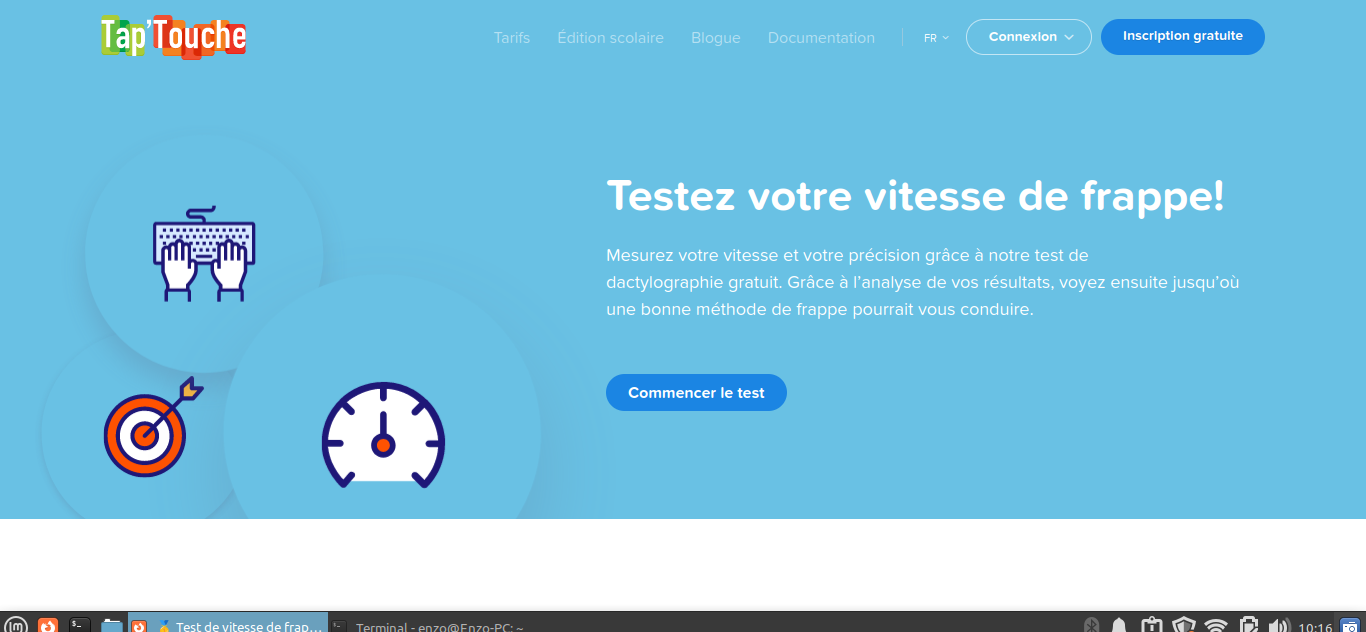
\includegraphics[width=\textwidth]{Image-TD-2/image_site_tap_touche.png}
    \caption{Page principale du site}
  \end{subfigure}
  \vspace{0.9cm} % Espace verticale entre les images
  \begin{subfigure}{0.45\textwidth}
    \centering
    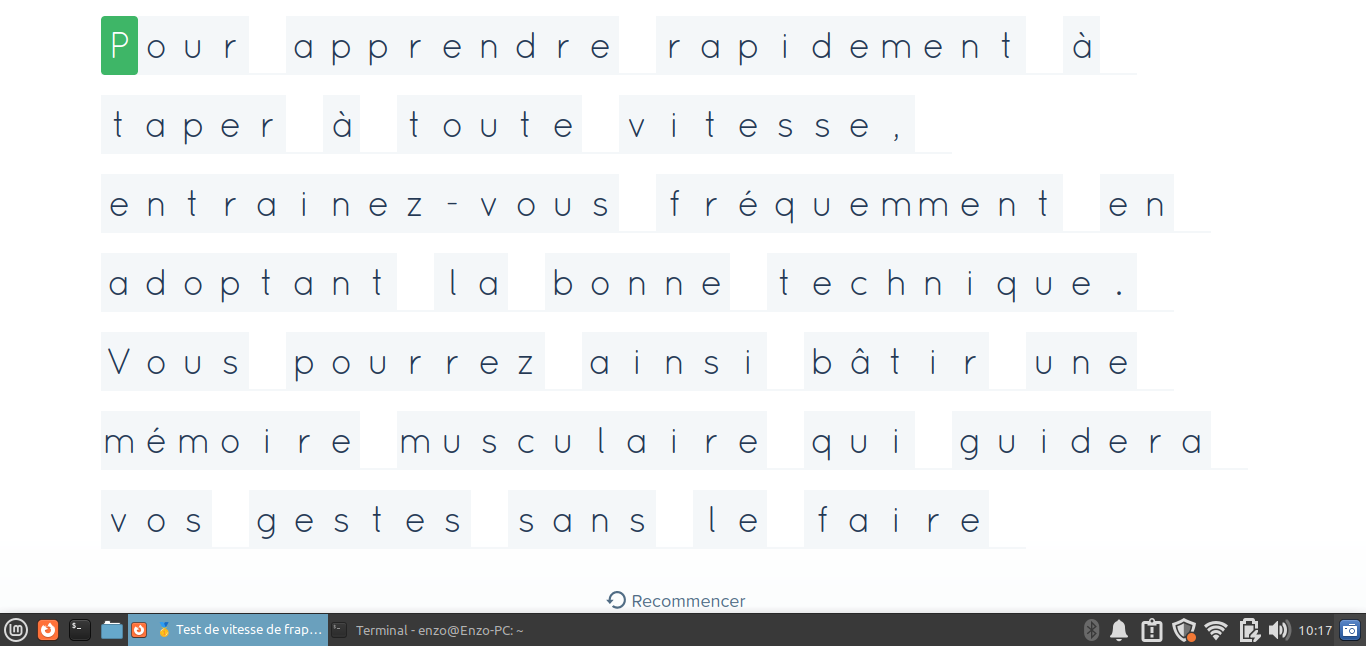
\includegraphics[width=\textwidth]{Image-TD-2/image_site_tap_touche2.png}
    \caption{Page pour effectuer le test de rapidité}
  \end{subfigure}
  \caption{Deux captures d'écran du site TapTouch}
\end{figure}

\vspace{0.3cm}

Essayer de masquer ses mains pour taper sans regarder

\vspace{0.3cm}

Inclure quelques résultats de rapidité.

\vspace{0.3cm}

Premier test effectué le 22/12/2022 : 

\begin{center}
  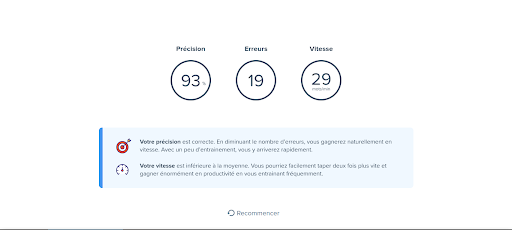
\includegraphics[width=10cm]{Image-TD-2/Premier_test.png}
\end{center}

\vspace{0.3cm}

\newpage

Deuxième test effectué le 23/12/2022 :

\begin{center}
  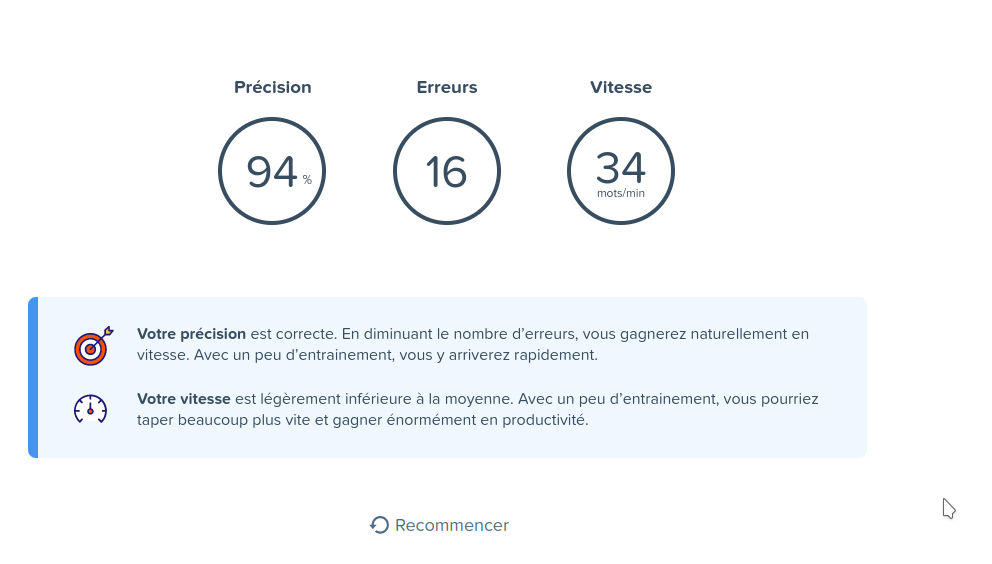
\includegraphics[width=10cm]{Image-TD-2/Deuxième_test.png}
\end{center}

\subsection{TD-3 : Vim et Emacs}

\begin{itemize}
  \item Effectuer les tutoriels pour Vim et Emacs :\\
  Vim : \texttt{vimtutor}\\
  Emacs : \texttt{emacs}, puis \texttt{Ctrl+H+T}
\end{itemize}

\vspace{0.3cm}

\begin{itemize}
  \item Paramétrer GNU Readline (le line editor par défault de bash) pour être en mode Emacs ou Vim
\end{itemize}

\vspace{0.3cm}

Une fois que j'ai effectué les deux tutoriels, je vais paramétrer GNU Readline en mode Vim. Pour ce faire, je vais utiliser la commande suivante :

\vspace{0.3cm}

\texttt{export EDITOR=vim}

\vspace{0.3cm}

Aprés, pour l'avoir de façon permanente, on peut ajouter cette ligne dans le fichier \texttt{~/.bashrc}.

\vspace{0.3cm}

\begin{itemize}
  \item Tester les deux 2 modes, en choisir un
\end{itemize}

\vspace{0.3cm}

J'ai testé ces deux modes et j'ai choisie d'utiliser Vim. 

\vspace{0.3cm}

\begin{itemize}
  \item Paramétrer Emacs ou Vim comme étant éditeur par défault en plus du mode Readline.
\end{itemize}

\vspace{0.3cm}

Pour qu'il soit de façon permanente, j'ai ajouté cette ligne suivante dans le fichier bashrc comme ci-dessous :

\vspace{0.3cm}

\begin{center}
  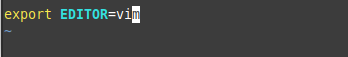
\includegraphics[width=10cm]{Image-TD-3/Ajout-ligne-bashrc.png}
\end{center}

\newpage

  \subsection{TD-4 : Commande history}

\begin{itemize}
  \item Regarder votre history
\end{itemize}

\vspace{0.3cm}

Voici ci-dessous, une capture d'écran de mon history : 

\begin{center}
  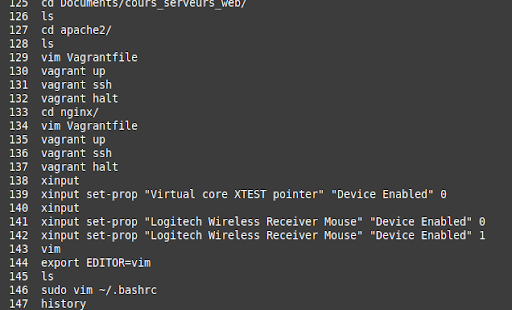
\includegraphics[width=10cm]{Image-TD-4/history.png}
\end{center}

\vspace{0.3cm}

\begin{itemize}
  \item Y a-t-il des informations sensible ? Comment y remédier ?
\end{itemize}

\vspace{0.3cm}

Oui, il peut y avoir des informations sensibles dans le history comme les mot de passe etc. Pour remédier à cela, nous pouvons utiliser un autre interpréteur de commande comme ZSH.

\vspace{0.3cm}

\begin{itemize}
  \item Un employé de longue date semble avoir un \texttt{history} très court, quelle sont les causes possibles ?\\
  \vspace{0.3cm}
  ~ cat ~/.bash\_history\\
  \vspace{0.3cm}
  sudo apt install curl zsh git\\
  \vspace{0.3cm}
  sh -c "(curl -fsSL https://raw.github.com/ohmyzsh/ohmyzsh/master/tools/install.sh)" 
\end{itemize}

\vspace{0.3cm}

On peut constater que cette employé à utiliser un autre interpréteur de commande qui est ZSH en le combinant avec OHMYZSH. Donc on ne peut plus voir son hisotry dans bash\_history.

\vspace{0.3cm}

\begin{itemize}
  \item Nos history sont souvent pollués par beaucoup de ls, cd, pwd ... Ces commandes sont tellement courtes que les taper entièrement est plus rapide. On veut éviter qu'elles n'apparaissent dans les résultats de recherche de l'history, comment faire ?
\end{itemize}

\vspace{0.3cm}

Pour eviter d'avoir certaine commande dans notre hisotry, on peut ajouter l'option \texttt{HISTIGNORE} dans le fichier bashrc : 

\vspace{0.3cm}

\begin{center}
  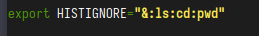
\includegraphics[width=10cm]{Image-TD-4/HISTIGNORE.png}
\end{center}

\vspace{0.3cm}

\newpage

Voici le resulat ci-dessous : 

\vspace{0.3cm}

\begin{figure}[h]
  \centering
  \begin{subfigure}{0.45\textwidth}
    \centering
    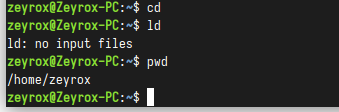
\includegraphics[width=\textwidth]{Image-TD-4/commande_test.png}
    \caption{Quelque commande pour tester HISTIGNORE}
  \end{subfigure}
  \vspace{0.9cm} % Espace verticale entre les images
  \begin{subfigure}{0.45\textwidth}
    \centering
    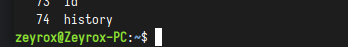
\includegraphics[width=\textwidth]{Image-TD-4/history1.png}
    \caption{Résultat dans history}
  \end{subfigure}
  \caption{Deux captures d'écran montrant un test de HISTIGNORE}
\end{figure}

\subsection{TD-5 : Alias}

\begin{itemize}
  \item Il est possible de créer des alias avec des arguments à l'aide des bash functions : 
\end{itemize}

\vspace{0.3cm}

Ecrire une bash function mkcd mondossier qui crée le dossier mondosser puis navigue dedans. 

\vspace{0.3cm}

Voici les étapes ci-dessous pour créer une bash function mkcd : 

\vspace{0.3cm}

\begin{center}
  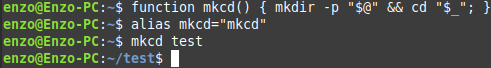
\includegraphics[width=10cm]{Image-TD-5/mkcd.png}
\end{center}

\vspace{0.3cm}

Ecrire une bash function gitemergency qui add, commit, et push tout son travail sur l'origine, permettant de ne rien perdre en cas d'alerte d'incendie.

\vspace{0.3cm}

Voici les étapes ci-dessous pour créer une bash function gitemergency : 

\vspace{0.3cm}

\begin{center}
  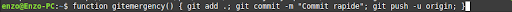
\includegraphics[width=14cm]{Image-TD-5/gitemergency.png}
\end{center}

\newpage

\subsection{TD-8 : Raccourci ZSH}

\vspace{0.3cm}

\begin{itemize}
  \item Dans zsh, créer un raccourci \texttt{Ctrl + Shift + A} :\\
  Lance les services apache et mariadb\\
  Log dans le terminal quand tout est lancé\\
  Ce reccourci est un interrupteur : apache et mariadb s'arrêtent si j'appuie à nouveau dessus.
\end{itemize}

\vspace{0.3cm}

Pour répondre à la question, nous allons tout d'abord crée un script bash comme ci-dessous : 

\vspace{0.3cm}

\begin{center}
  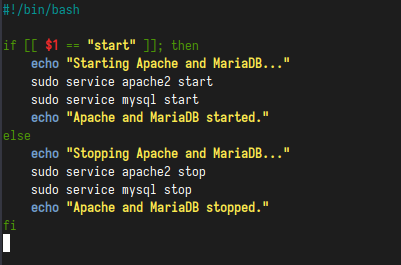
\includegraphics[width=7cm]{Image-TD-8/Sevices.png}
\end{center}

\vspace{0.3cm}

Maintenant que nous avons crée le scrpite .sh, nous allons crée deux fonctions dans le fichier .zshrc pour faire fonctionner le script comme ci-dessous : 

\vspace{0.3cm}

\begin{center}
  \includegraphics[width=7cm]{Image-TD-8/fonction\_zsh.png}
\end{center}

\vspace{0.3cm}

Maintenant que nous avons crée les deux fonctions, nous allons les combinaison de touche dans le fichier .zshrc comme ci-dessous : 

\vspace{0.3cm}

\begin{center}
  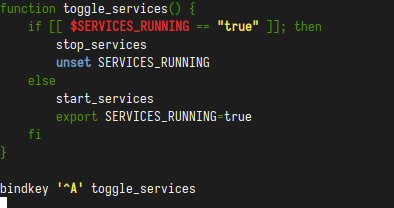
\includegraphics[width=7cm]{Image-TD-8/bindkey.png}
\end{center}

\vspace{0.3cm}

Il nous reste plus qu'à utiliser la commande \texttt{source ~/.zshrc} pour que les modification soient prises en comptes.

\end{document}

